\documentclass{beamer}

\usetheme{CambridgeUS}
\usecolortheme{beaver}

\usepackage[utf8]{inputenc}
\usepackage[brazil]{babel}
\usepackage{caption}
% \usepackage{hyperref}
\hypersetup{
    final=true,
    bookmarks=true,
    unicode=false,          % non-Latin characters in Acrobat’s bookmarks
    pdftoolbar=true,        % show Acrobat’s toolbar?
    pdfmenubar=true,        % show Acrobat’s menu?
    pdffitwindow=false,     % window fit to page when opened
    pdfstartview={FitH},    % fits the width of the page to the window
    pdftitle={Introdução ao \LaTeX com o Visual Studio Code no Windows},    % title
    pdfauthor={Nightwind},     % author
    pdfsubject={Introdução ao Visual Studio Code no Windows},   % subject of the document
    % pdfcreator={Creator},   % creator of the document
    % pdfproducer={Producer}, % producer of the document
    pdfkeywords={latex, dicas}, % list of keywords
    pdfnewwindow=true,      % links in new PDF window
    colorlinks=false,       % false: boxed links; true: colored links
    linkcolor=red,          % color of internal links (change box color with linkbordercolor)
    citecolor=green,        % color of links to bibliography
    filecolor=cyan,         % color of file links
    urlcolor=magenta        % color of external links
}
\usepackage[style=abnt]{biblatex}
\addbibresource{references.bib}
\usepackage{csquotes}

\usepackage{xcolor}
\usepackage{listings}
\lstset
{breakatwhitespace=true,breaklines=true,language=[LaTeX]TeX,basicstyle=\small\ttfamily,flexiblecolumns,backgroundcolor=\color{white}}

\title{Utilizando o Visual Studio Code no Windows}
\author{Nightwind}
\institute[CTISM]{Colégio Técnico Industrial de Santa Maria}
\logo{
\includegraphics[width=1cm]{../images/photo1.jpg}}
\date{\today}

\begin{document}

\frame{\titlepage}

\begin{frame}
    \frametitle{Sumário}
    \tableofcontents
\end{frame}

\section{Introdução}
\begin{frame}
    \frametitle{Introdução}

    \begin{itemize}
        \item O Visual Studio Code é um editor de código \textit{open-source} e gratuito.
        \item Funciona no Windows, Linux e macOS.
        \item Suporta muitas linguagens de programação.
        \begin{itemize}
            \item Só precisa baixar a extensão da linguagem e os pré-requisitos das extensões.
        \end{itemize}
    \end{itemize}

\end{frame}

\section{Instalação do Visual Studio Code}

\begin{frame}
    \frametitle{Instalação do Visual Studio Code}
    \begin{enumerate}
        \item Acessar o site oficial: \href{https://code.visualstudio.com/Download}{Visual Studio Code}
        \item Fazer o download e seguir os passos da instalação padrão: aceitar os termos de uso, determinar o local de instalação, atalho no Menu Iniciar, selecionar as tarefas adicionais e confirmar as opções pedidas.
    \end{enumerate}
\end{frame}

\begin{frame}
    \frametitle{Instalação do Visual Studio Code}
\begin{figure}[h]
    \centering
    \caption{Contrato dos Termos de Uso.}
    \label{fig:contrato}
    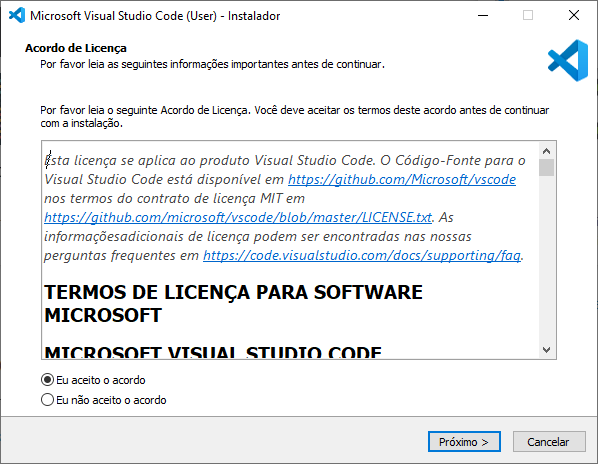
\includegraphics[width=0.8\textheight]{../images/contrato.png}
    \caption*{\footnotesize Leia e aceite o acordo.}
\end{figure}
\end{frame}

\begin{frame}
    \frametitle{Instalação do Visual Studio Code}
\begin{figure}[h]
    \centering
    \caption{Local de instalação.}
    \label{fig:local}
    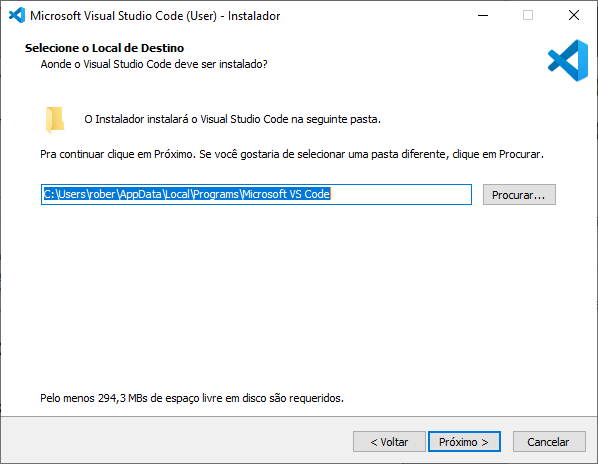
\includegraphics[width=0.8\textheight]{../images/local.png}
    \caption*{\footnotesize Escolha a partição e a pasta que deseja instalar.}
\end{figure}
\end{frame}

\begin{frame}
    \frametitle{Instalação do Visual Studio Code}
\begin{figure}[h]
    \centering
    \caption{Atalho no Menu Iniciar.}
    \label{fig:atalho_menu_iniciar}
    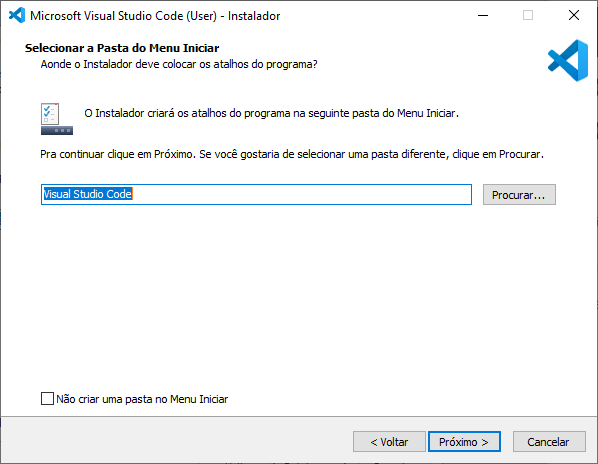
\includegraphics[width=0.8\textheight]{../images/atalho_menu_iniciar.png}
    \caption*{\footnotesize Se desejar incluir um atalho no menu iniciar, determine o nome da pasta.}
\end{figure}
\end{frame}

\begin{frame}
    \frametitle{Instalação do Visual Studio Code}
\begin{figure}[h]
    \centering
    \caption{Tarefas Adicionais.}
    \label{fig:tarefas_adicionais}
    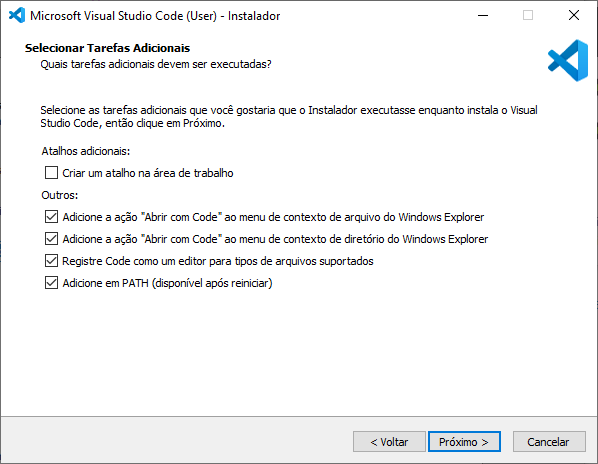
\includegraphics[width=0.8\textheight]{../images/tarefas adicionais.png}
    \caption*{\footnotesize Sugere-se que, no mínimo, a segunda, terceira e quarta opções sejam marcadas.}
\end{figure}
\end{frame}

\begin{frame}
    \frametitle{Instalação do Visual Studio Code}
\begin{figure}[h]
    \centering
    \caption{Confirmação de instalação.}
    \label{fig:verificador_instalacao}
    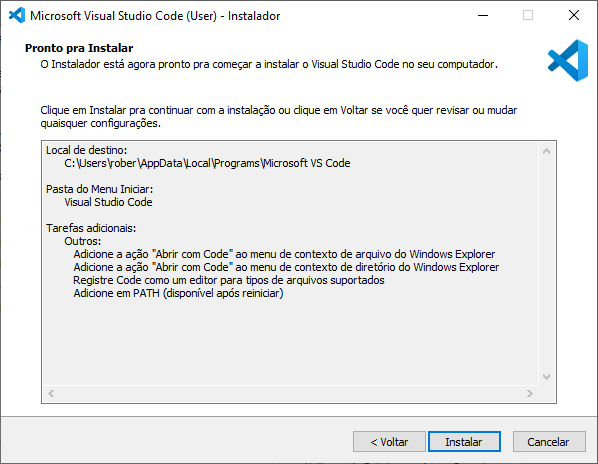
\includegraphics[width=0.75\textheight]{../images/verificador_instalação.png}
    \caption*{\footnotesize Leia atentamente e clique em ``Instalar'' caso esteja tudo certo. Senão volte nas configurações que deseja alterar.}
\end{figure}
\end{frame}

\section{Configurações Iniciais}
\begin{frame}
    \frametitle{Configurações Iniciais}
\begin{itemize}
    \item Quando o Visual Studio Code foi iniciado pela primeira vez, uma tela de configurações e sugestões iniciais irá aparecer. 
    \item Nesta parte, espera-se que o usuário edite o Visual Studio Code de acordo com as suas necessidades.
    \item Editar o tema, inserir as extensões que deseja, verificar os atalhos e abrir o primeiro arquivo.
\end{itemize}
\end{frame}

\begin{frame}
    \frametitle{Configurações Iniciais}
\begin{figure}[h]
    \centering
    \caption{Tela de boas-vindas.}
    \label{fig:welcome_page}
    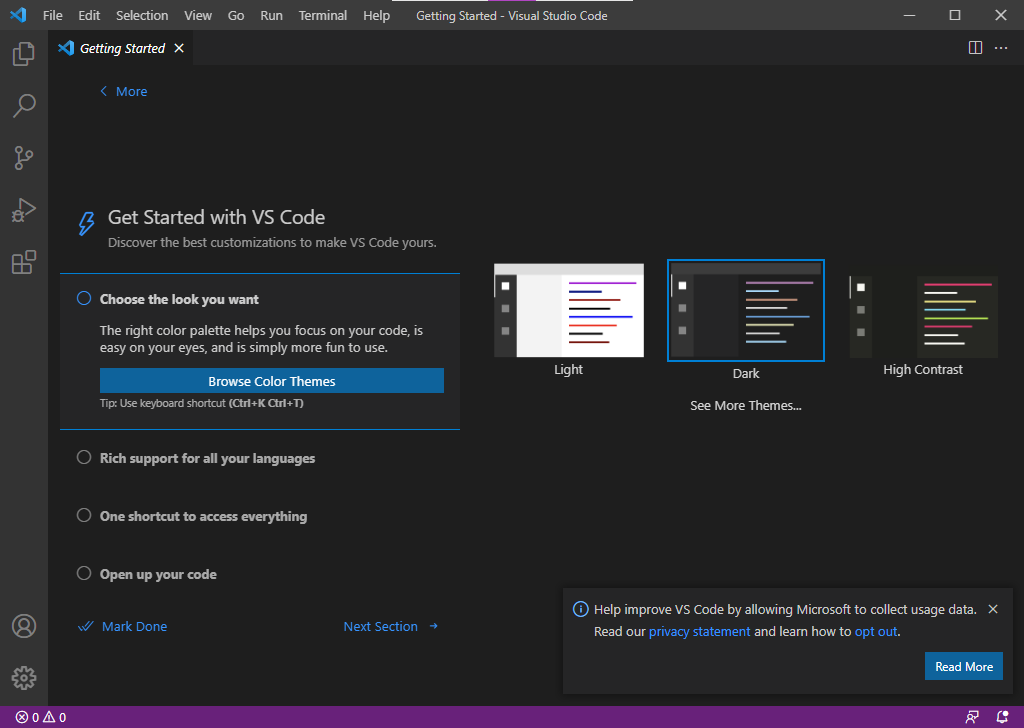
\includegraphics[width=0.8\textheight]{../images/welcome_page.png}
    \caption*{\footnotesize Adapte-se com a aparência. Siga as sugestões de inicialização.}
\end{figure}
\end{frame}

\begin{frame}
    \frametitle{Configurações Iniciais}
\begin{figure}[h]
    \centering
    \caption{Extensões sugeridas.}
    \label{fig:extensoes}
    \includegraphics[width=0.8\textheight]{../images/extensões.png}
    \caption*{\footnotesize Observar que o ícone de extensões está sempre no lado esquerdo da tela. Sempre que precisar instalar uma extensão, clicar nele.}
\end{figure}
\end{frame}

\begin{frame}
    \frametitle{Configurações Iniciais}
\begin{figure}[h]
    \centering
    \caption{Extensão para arquivos \LaTeX.}
    \label{fig:LaTeX_Workshop}
    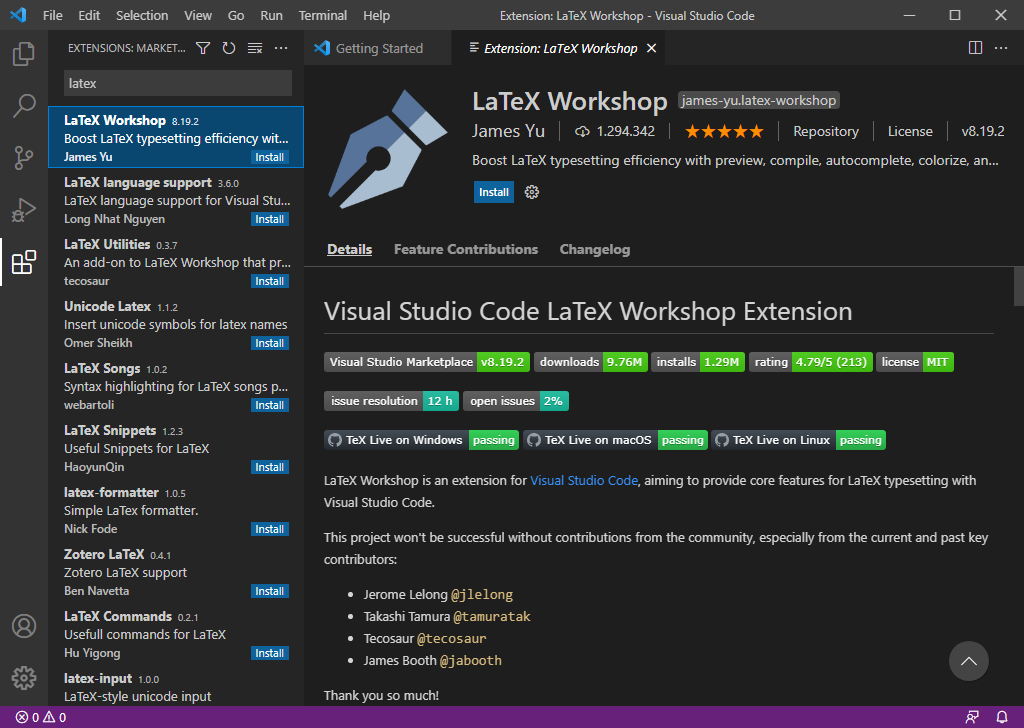
\includegraphics[width=0.8\textheight]{../images/LaTeX_Workshop.png}
    \caption*{\footnotesize Escrever na caixa de pesquisa ``latex'' e instalar está opção que está ilustrada.}
\end{figure}
\end{frame}

\begin{frame}
    \frametitle{Configurações Iniciais}
\begin{figure}[h]
    \centering
    \caption{Extensão para corrigir os erros de Português (BR).}
    \label{fig:brazilian_portuguese_spell-checker}
    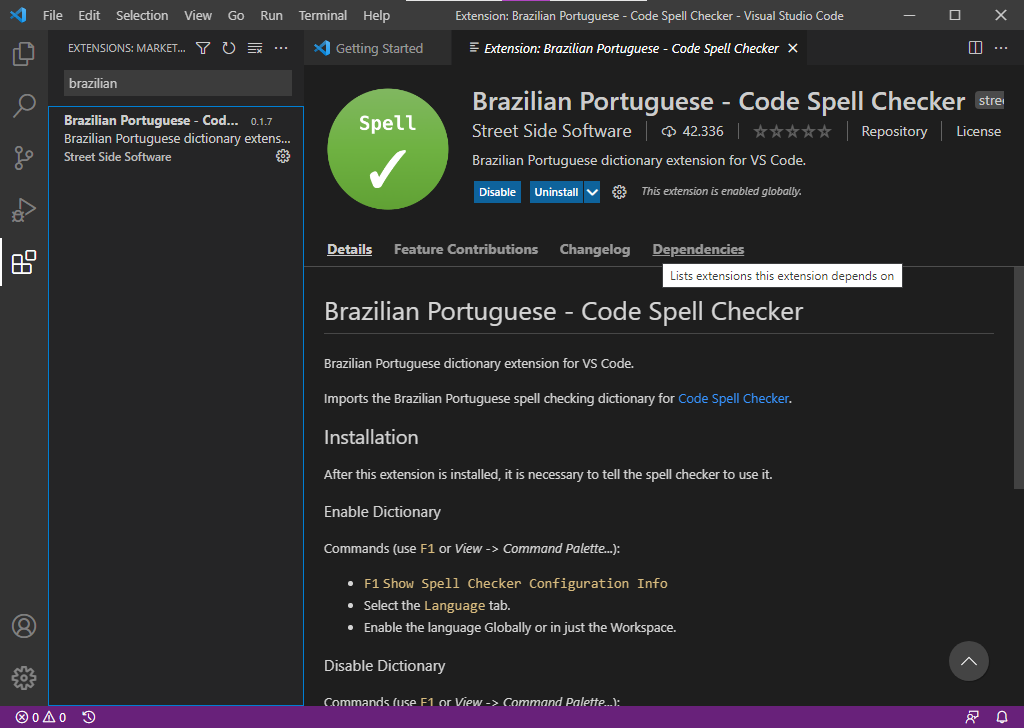
\includegraphics[width=0.8\textheight]{../images/brazilian_portuguese_spell-checker.png}
    \caption*{\footnotesize Sugestão: instalar esta extensão para que erros muito esdrúxulos não passem.}
\end{figure}
\end{frame}

\begin{frame}
    \frametitle{Configurações Iniciais}
\begin{figure}[h]
    \centering
    \caption{Atalhos.}
    \label{fig:atalhos}
    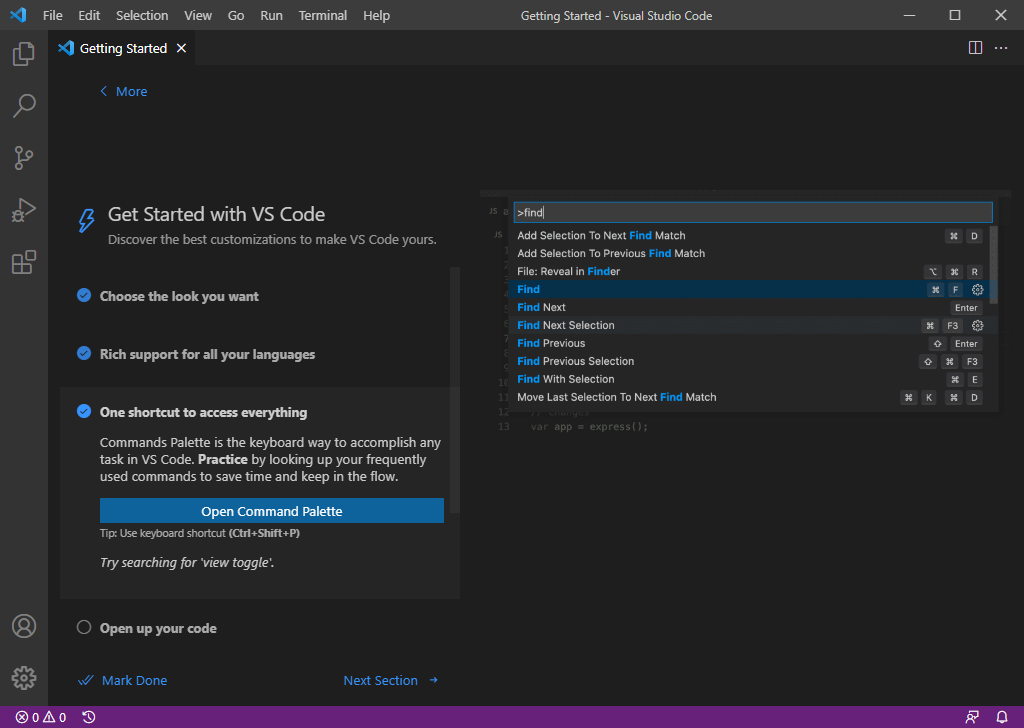
\includegraphics[width=0.8\textheight]{../images/atalhos.png}
    \caption*{\footnotesize ctrl+shift+P.}
\end{figure}
\end{frame}

\section{Instalação dos Requisitos}

\begin{frame}
    \frametitle{Instalação dos Requisitos}
    \begin{itemize}
        \item O requisito para que se possa compilar um arquivo LaTeX no Visual Studio Code é visto na documentação do Latex-Workshop.
        \item Nela, há a recomendação de que a TeXLive seja baixada e instalada previamente para que um documento LaTeX possa ser compilado no Visual Studio Code.
    \end{itemize}
\end{frame}

\begin{frame}
    \frametitle{Configurações Iniciais}
\begin{figure}[h]
    \centering
    \caption{TeXLive.}
    \label{fig:texlive}
    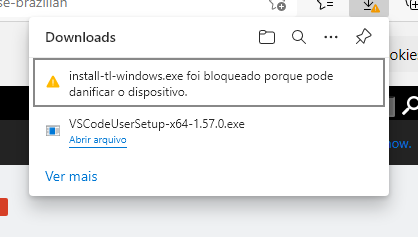
\includegraphics[width=0.8\textheight]{../images/texlive.png}
    \caption*{\footnotesize Ir no \href{https://www.tug.org/texlive/acquire-netinstall.html}{Site oficial} e clicar no texto destacado \href{https://mirror.ctan.org/systems/texlive/tlnet/install-tl-windows.exe}{\underline{install-tl-windows.exe}}.} 
\end{figure}
\end{frame}

\begin{frame}
    \frametitle{Instalação dos Requisitos}
    \begin{itemize}
        \item Quando o Download for concluído, aparecerá um aviso de que o software poderá causar danos ao PC. Mas ele não causa. Pode continuar com a instalação.
    \end{itemize}
\end{frame}

\begin{frame}
    \frametitle{Configurações Iniciais}
\begin{figure}[h]
    \centering
    \caption{Instalação da TeXLive.}
    \label{fig:instalador}
    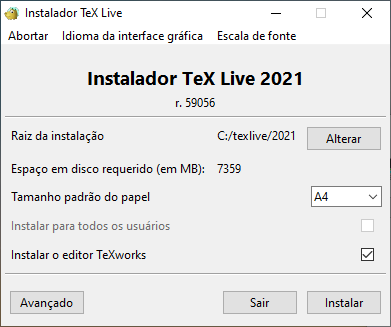
\includegraphics[width=0.5\textheight]{../images/instalador.png}
    \caption*{\footnotesize  Clicar em ``Instalar'' e aguardar. Pode demorar bastante, instale quando tiver tempo para esperar um processo longo.}
\end{figure}
\end{frame}

\begin{frame}[fragile]
    \frametitle{Instalação dos Requisitos}
    \begin{itemize}
        \item Depois de pronto, pode-se fazer um pequeno teste.
        \begin{enumerate}
            \item Criar um novo arquivo.
            \item Nomeá-lo como ``teste.tex'' e escrever: 
            \begin{lstlisting}[language=TeX]
                \documentclass{article}
                \begin{document}
                    Ola!
                \end{document}
            \end{lstlisting}
            \item Apertar no botãozinho que tem uma setinha para a direita verde para que o pdf seja gerado.
            \item Apertar no quadrinho que tem uma lupinha na frete para ver o pdf.
        \end{enumerate}
    \end{itemize}
\end{frame}

\begin{frame}
    \frametitle{Configurações Iniciais}
\begin{figure}[h]
    \centering
    \caption{Arquivo Teste.}
    \label{fig:arquivo-pronto}
    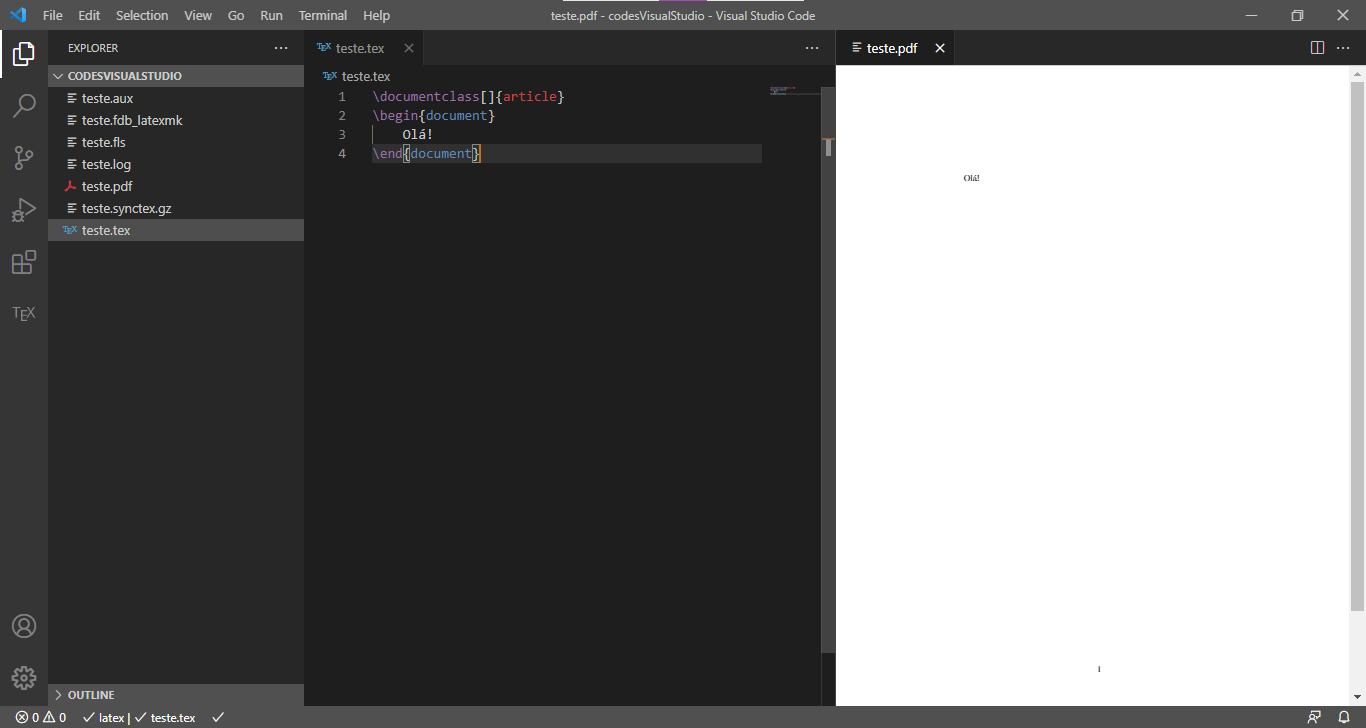
\includegraphics[width=0.8\textheight]{../images/arquivo-pronto.png}
    \caption*{\footnotesize  Demonstração do resultado final.}
\end{figure}
\end{frame}

\section{Referências}

\begin{frame}[allowframebreaks]
    \frametitle{Referências}
    \nocite{LaTeXWorkshop,TeXLiveHomePage,VisualStudioCode}
    \printbibliography[]
\end{frame}

\end{document}
